\subsection{Lab8: Receptor FM Mono}
%*********************
\begin{frame}{}

\pgfdeclareimage[width=\paperwidth,height=\paperheight]{bg}{imagenes/fondo_lab}
\setbeamertemplate{background}{\pgfuseimage{bg}}

\bfseries{\textrm{\LARGE Lab8\\ \Large Receptor FM Monofónico}}
\raggedright
\end{frame}
%*********************

\begin{frame}{Diagrama del receptor FM Monofónico}

\pgfdeclareimage[width=\paperwidth,height=\paperheight]{bg}{imagenes/fondo3}
\setbeamertemplate{background}{\pgfuseimage{bg}}

\begin{figure}[H]
\centering
\vspace{-3mm}
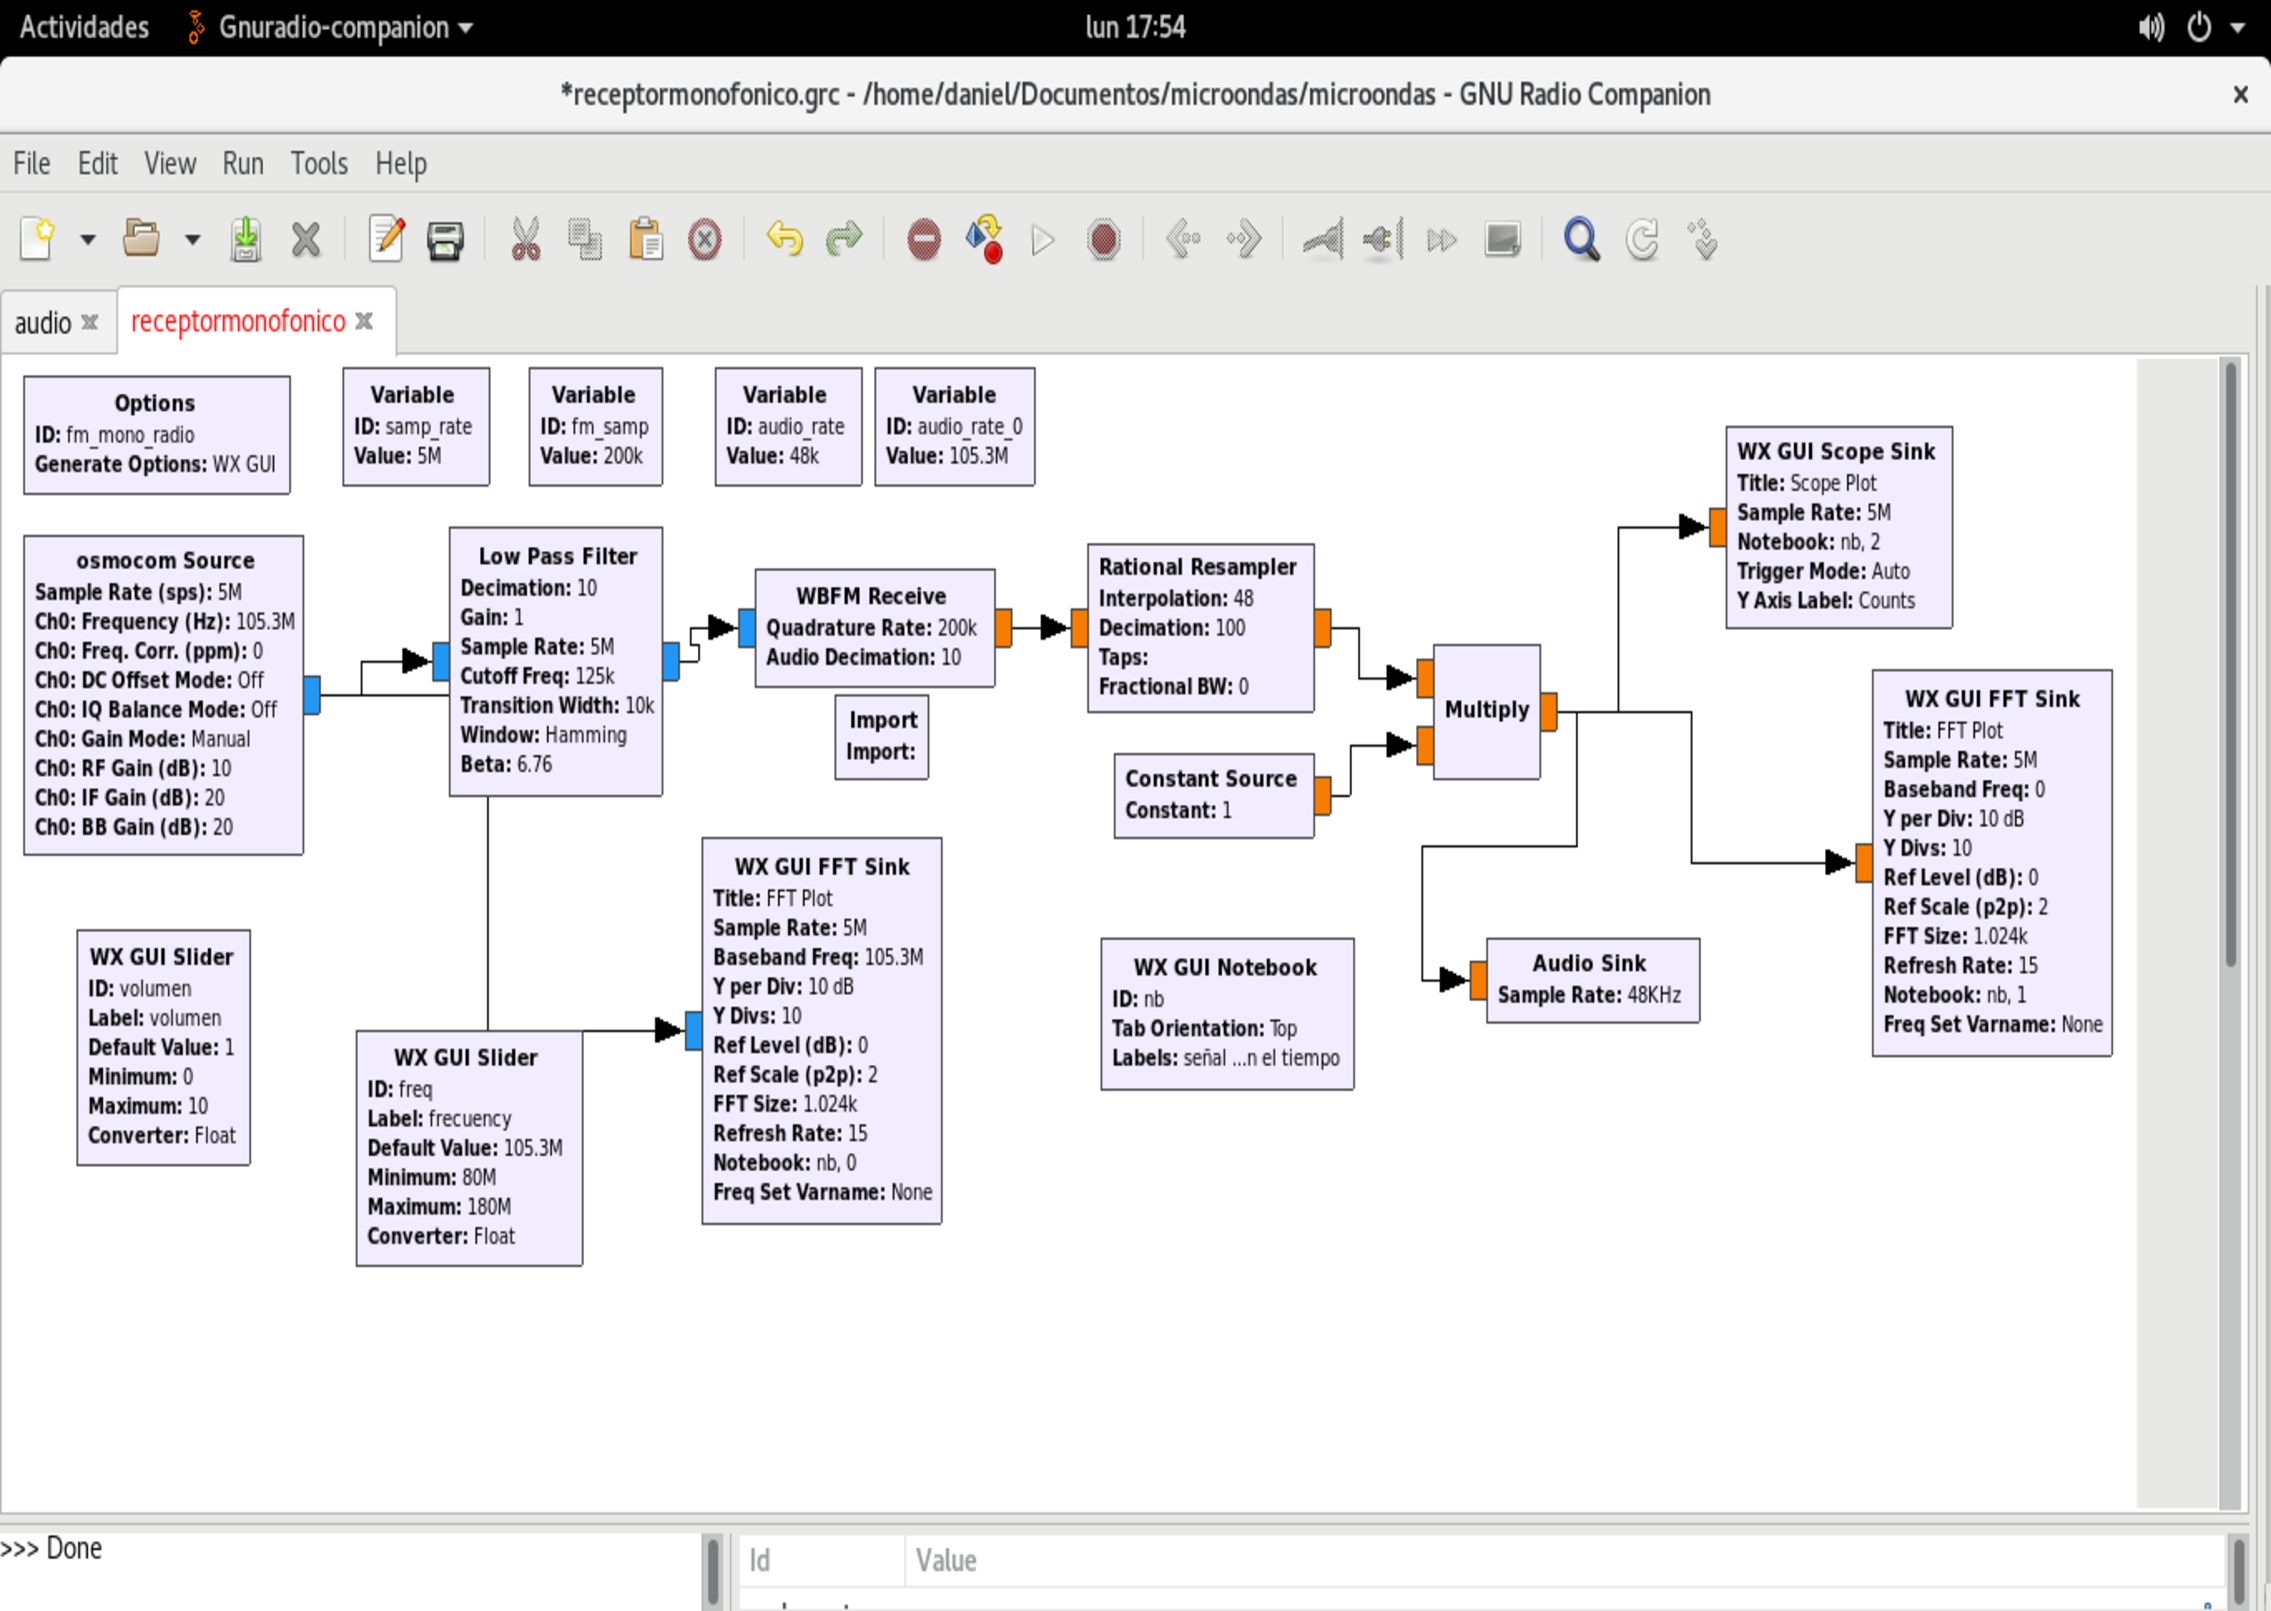
\includegraphics[width=\textwidth]{parte3/lab8/pdf/lab8_1.pdf}
\end{figure}

\end{frame}
%---------------------------------

\begin{frame}{Receptor FM Monofónico}

\begin{figure}[H]
\centering
\vspace{-3mm}
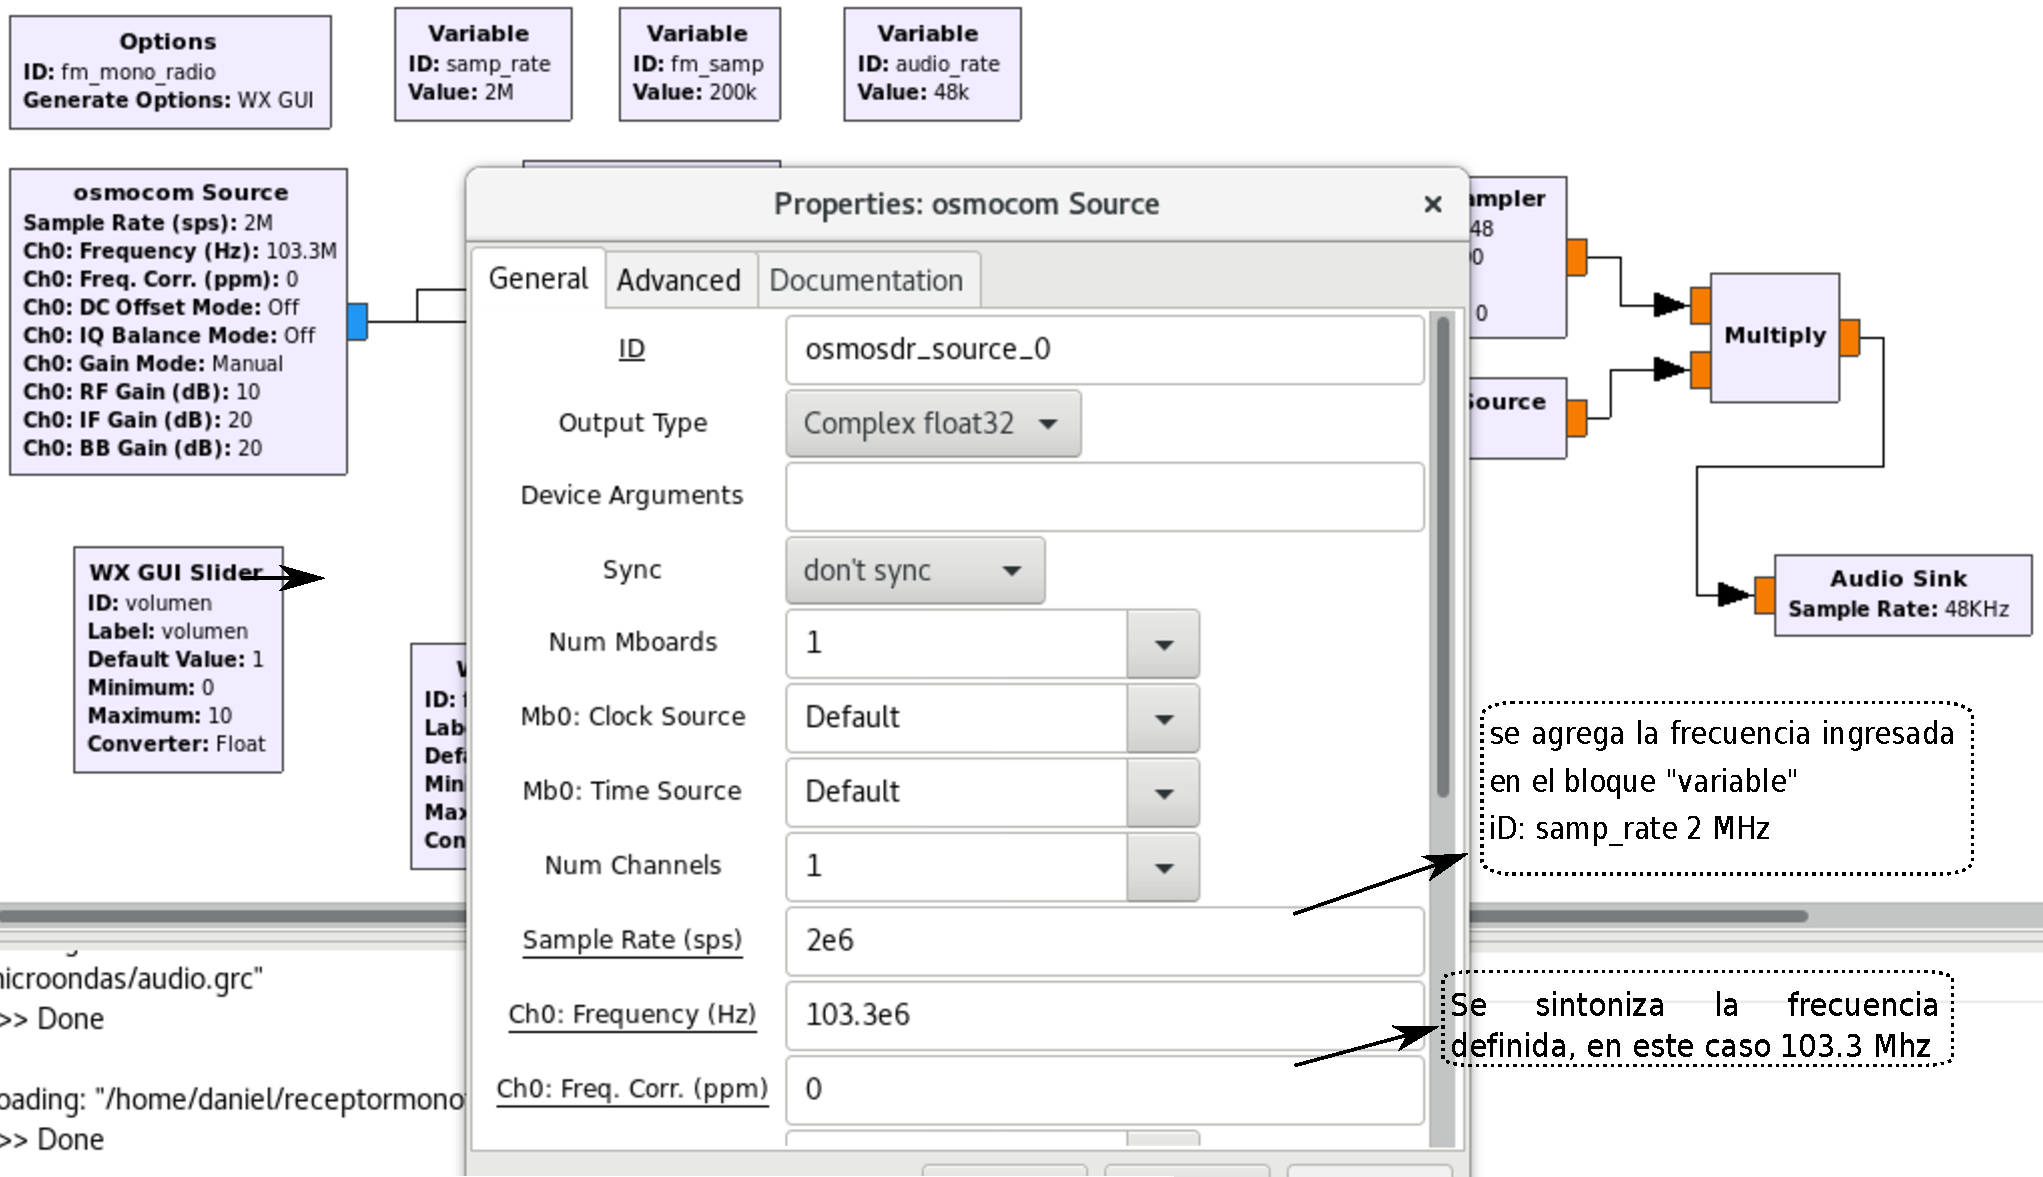
\includegraphics[width=\textwidth]{parte3/lab8/pdf/lab8_2.pdf}
\end{figure}

\end{frame}
%---------------------------------

\begin{frame}{Receptor FM Monofónico}

\begin{figure}[H]
\centering
\vspace{-3mm}
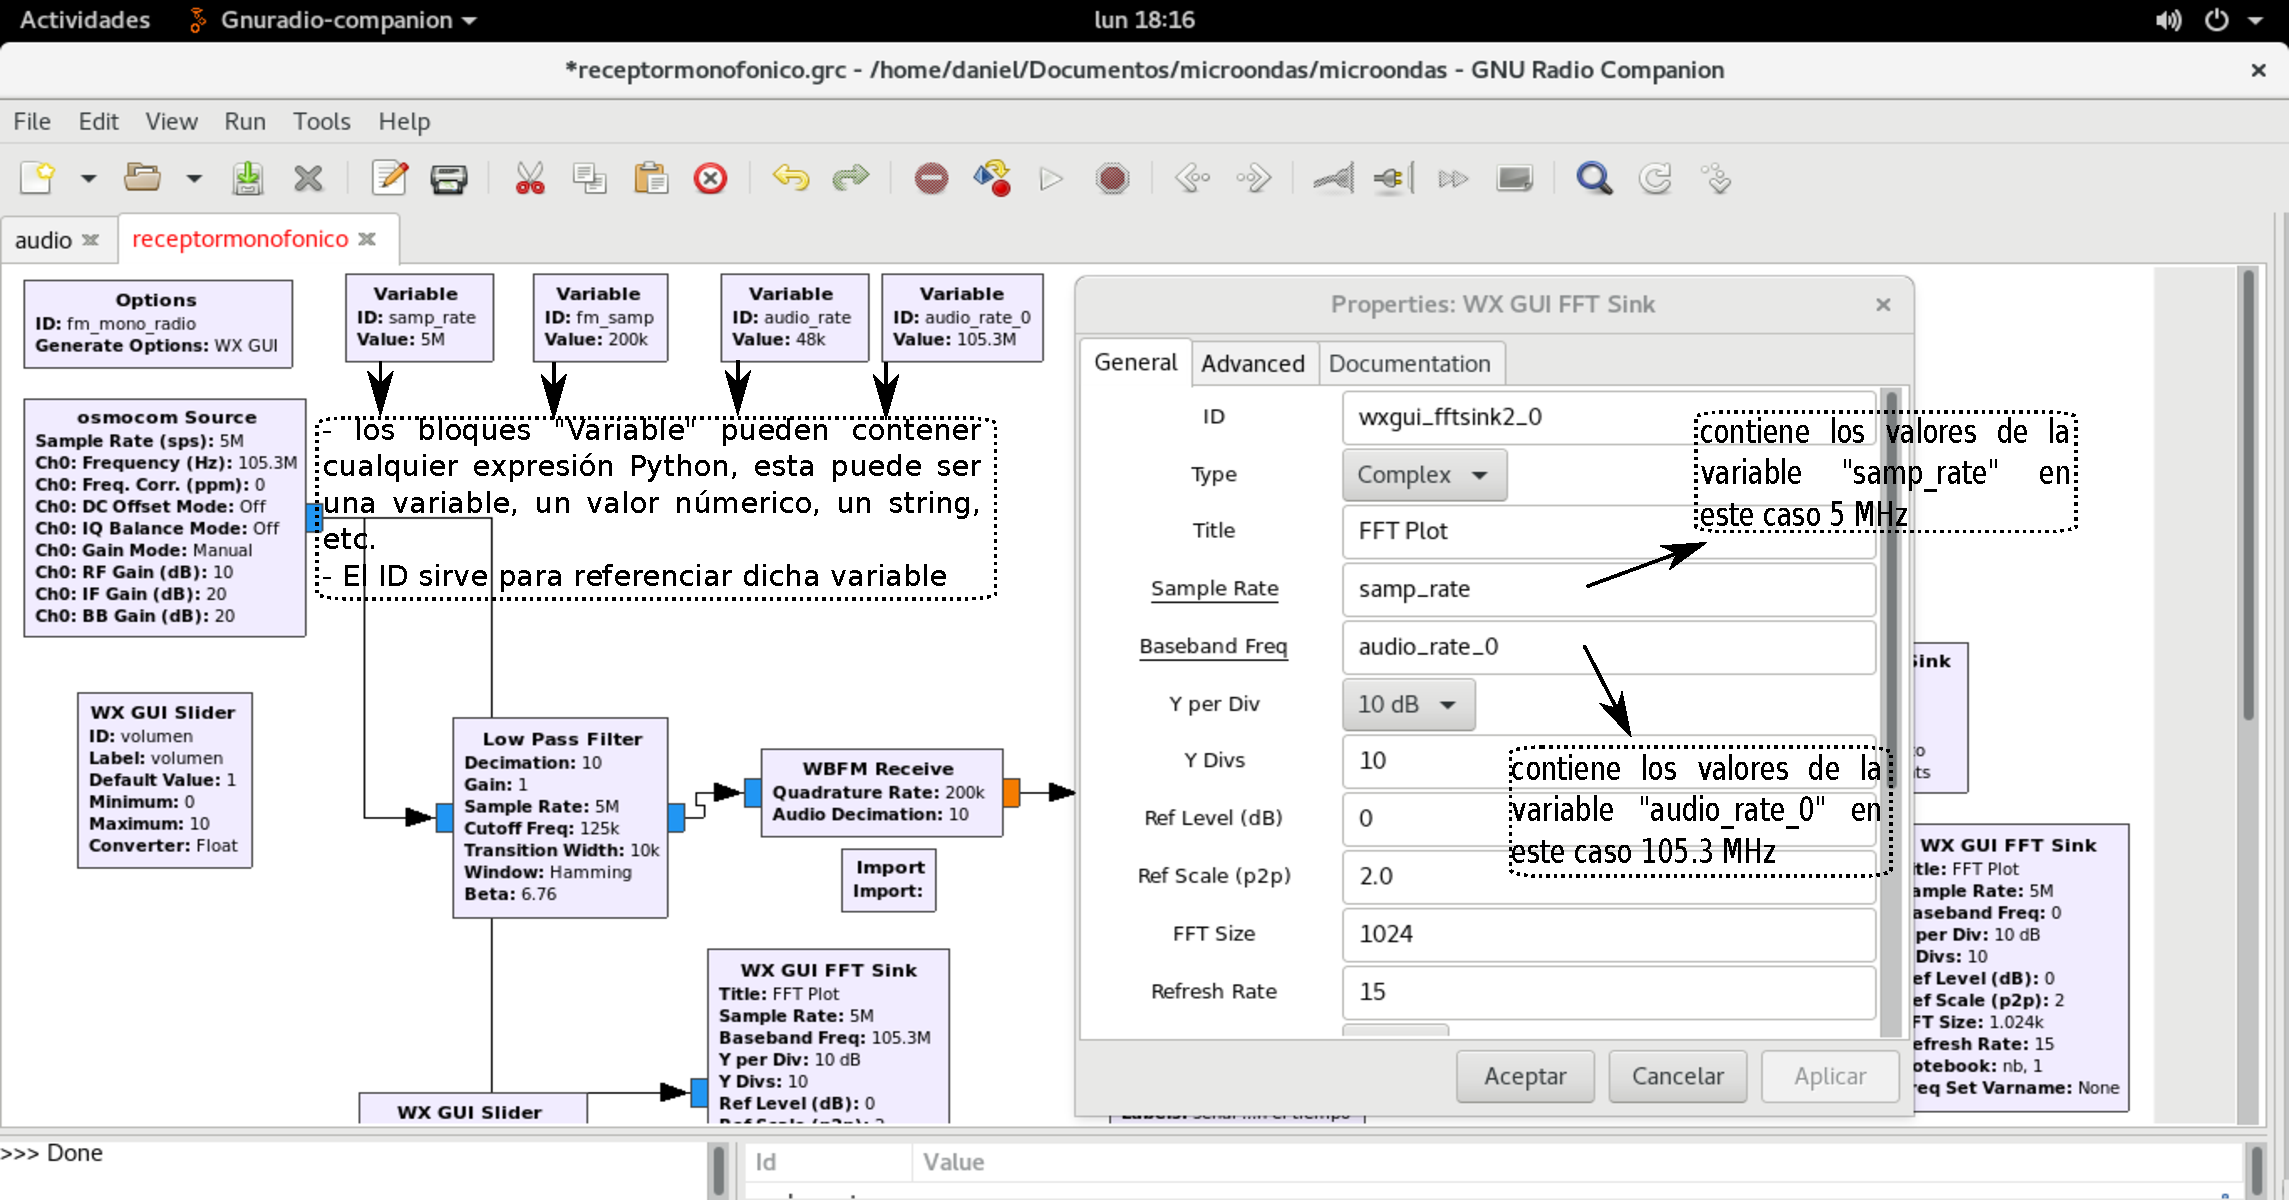
\includegraphics[width=\textwidth]{parte3/lab8/pdf/lab8_3.pdf}
\end{figure}

\end{frame}
%---------------------------------

\begin{frame}{Receptor FM Monofónico}

\begin{figure}[H]
\centering
\vspace{-3mm}
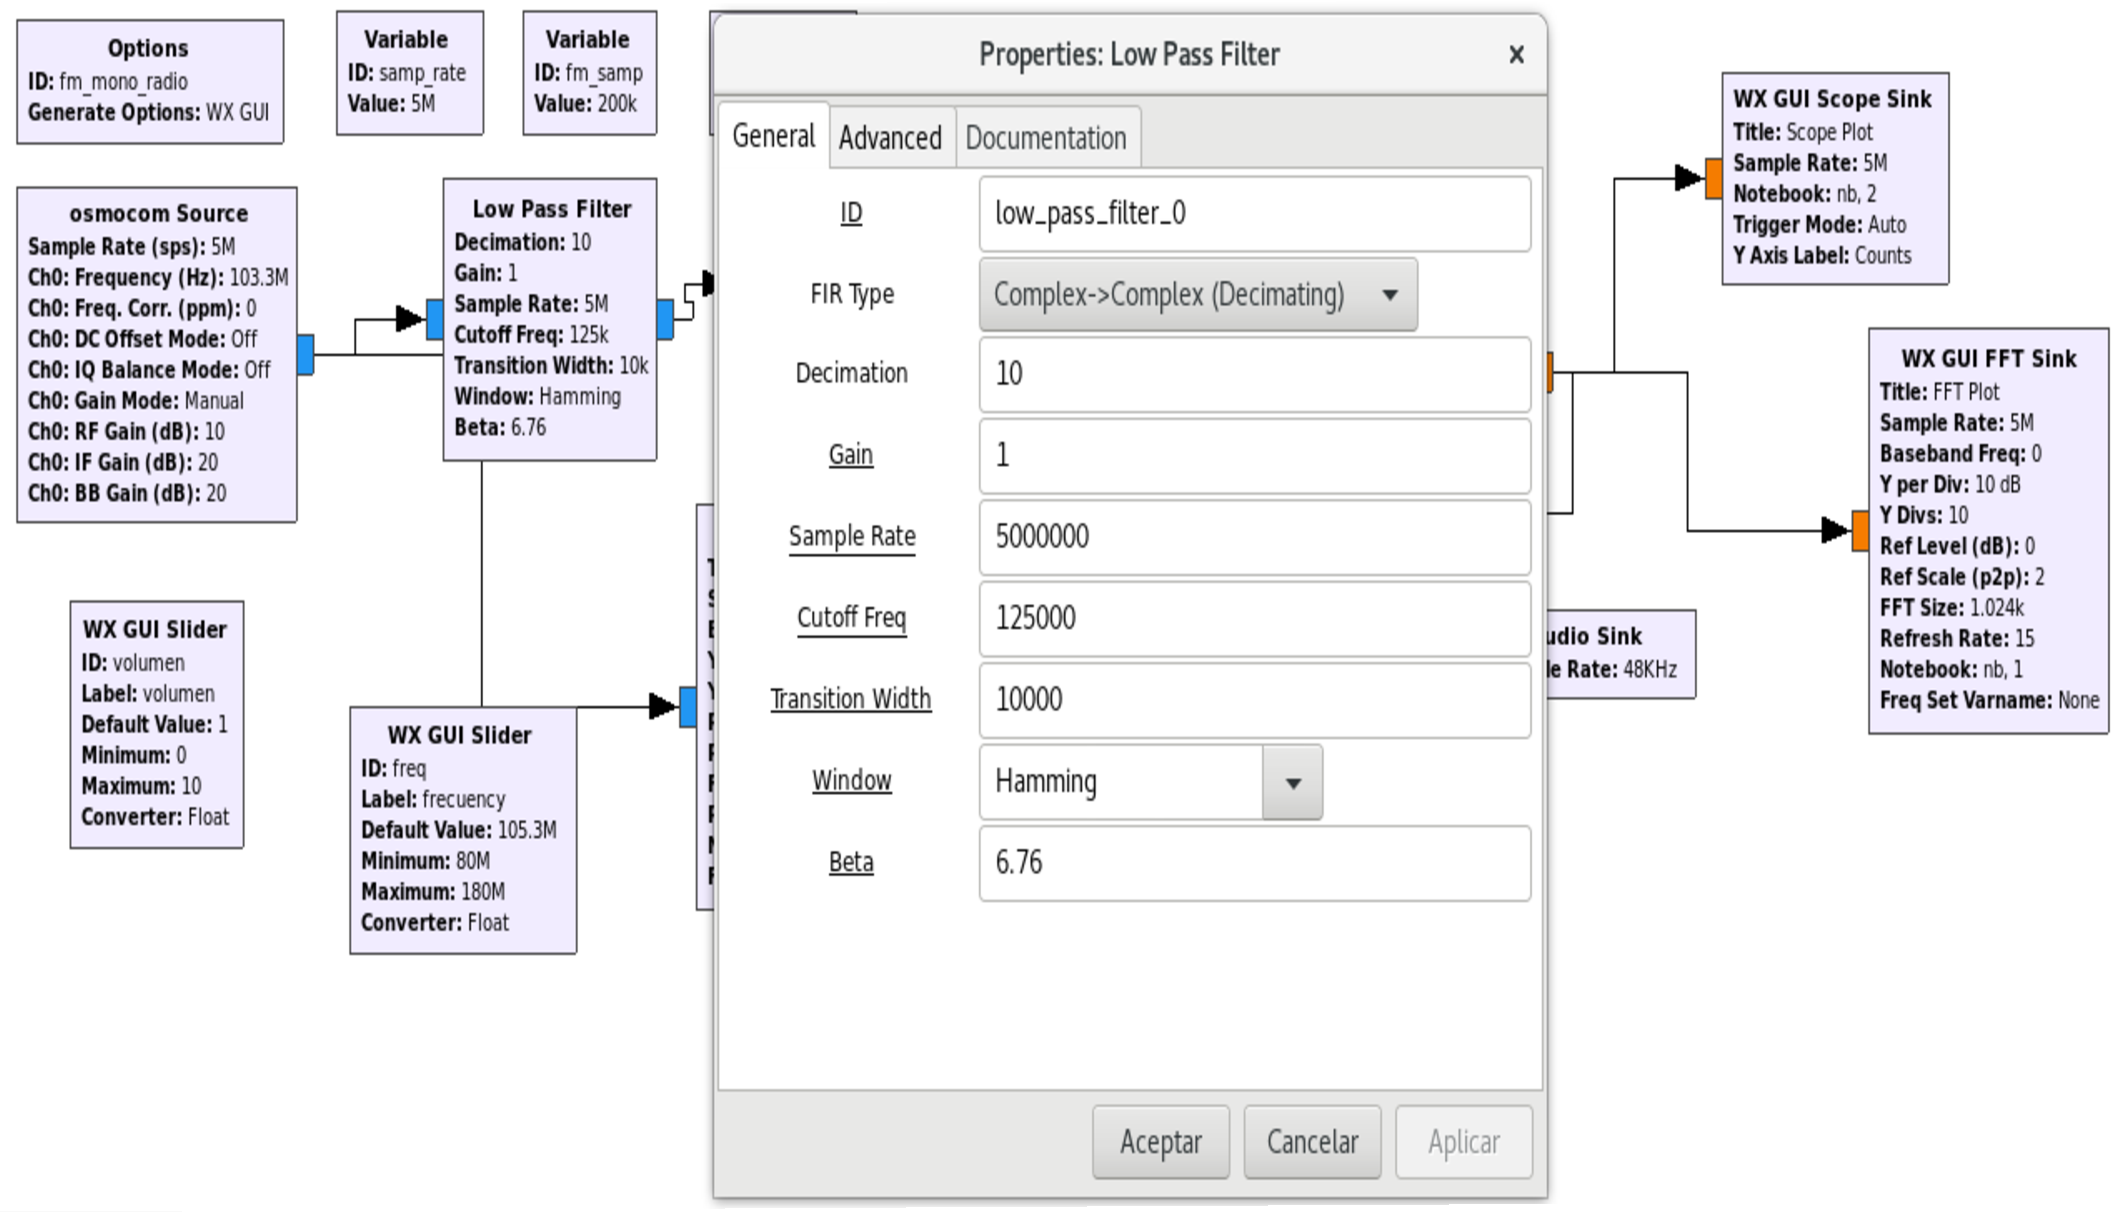
\includegraphics[width=\textwidth]{parte3/lab8/pdf/lab8_4.pdf}
\end{figure}

\end{frame}
%---------------------------------

\begin{frame}{Receptor FM Monofónico}

\begin{figure}[H]
\centering
\vspace{-3mm}
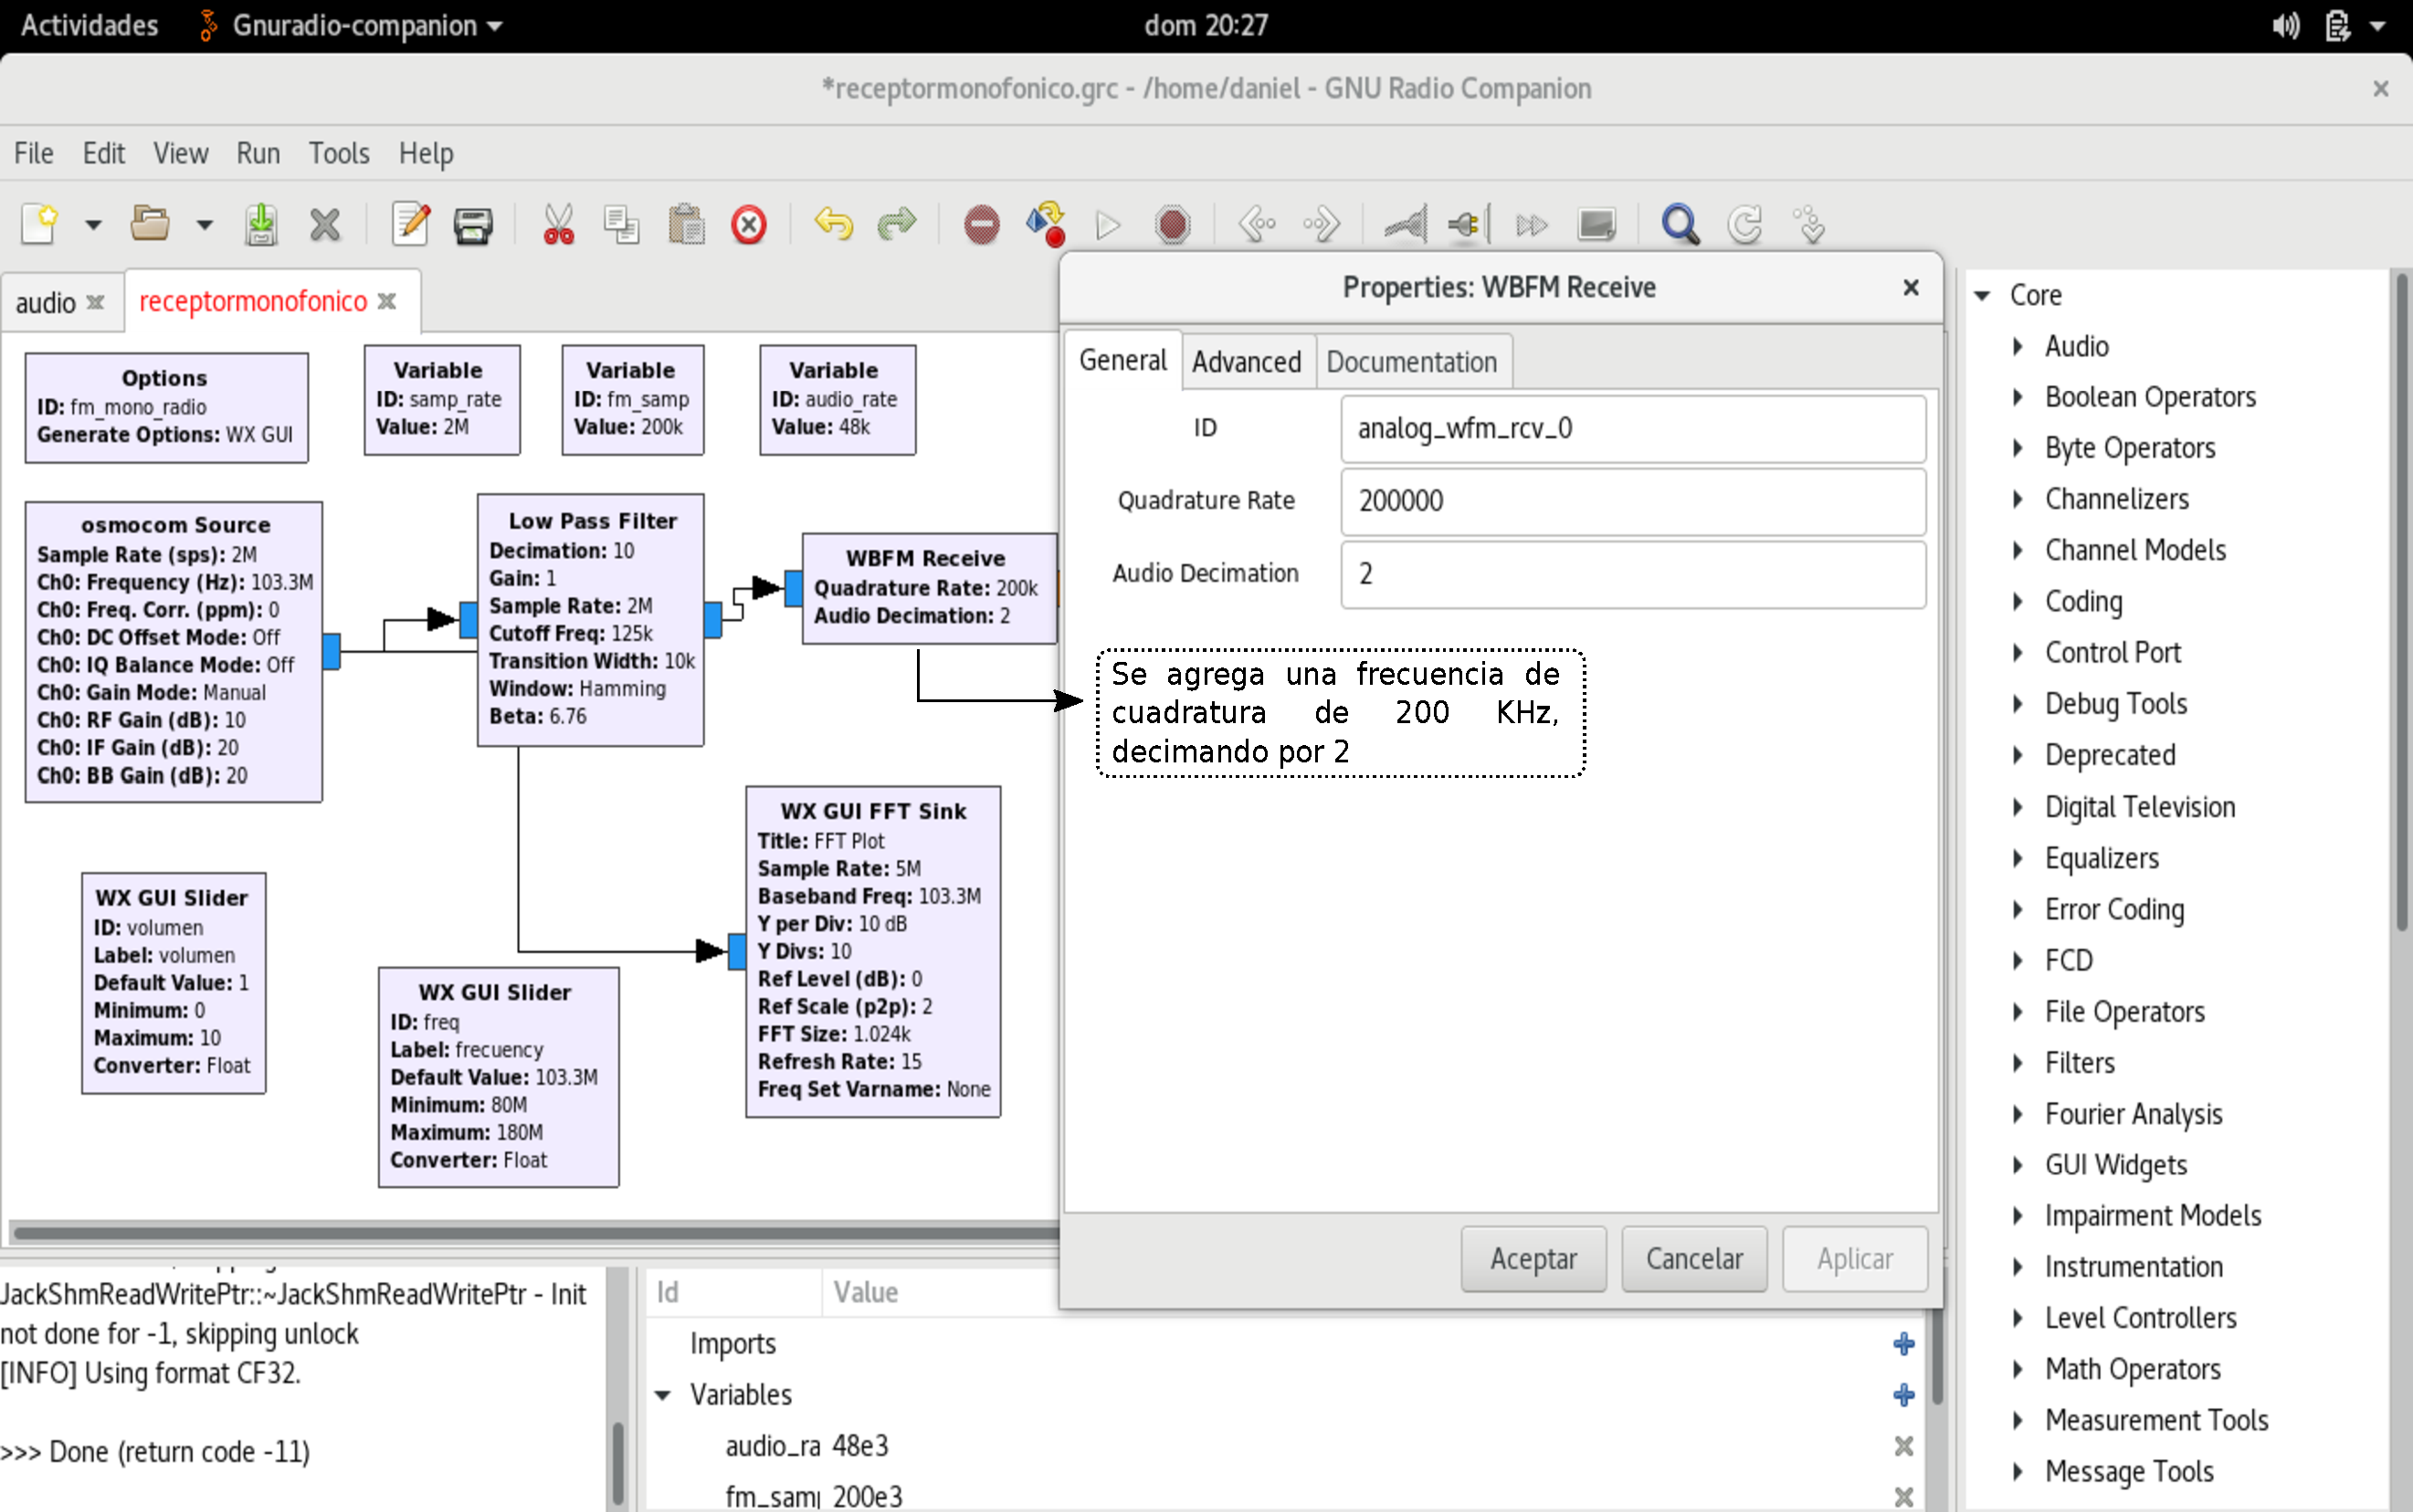
\includegraphics[width=\textwidth]{parte3/lab8/pdf/lab8_5.pdf}
\end{figure}

\end{frame}
%---------------------------------

\begin{frame}{Proceso matemático}

\begin{figure}[H]
\centering
\vspace{-3mm}
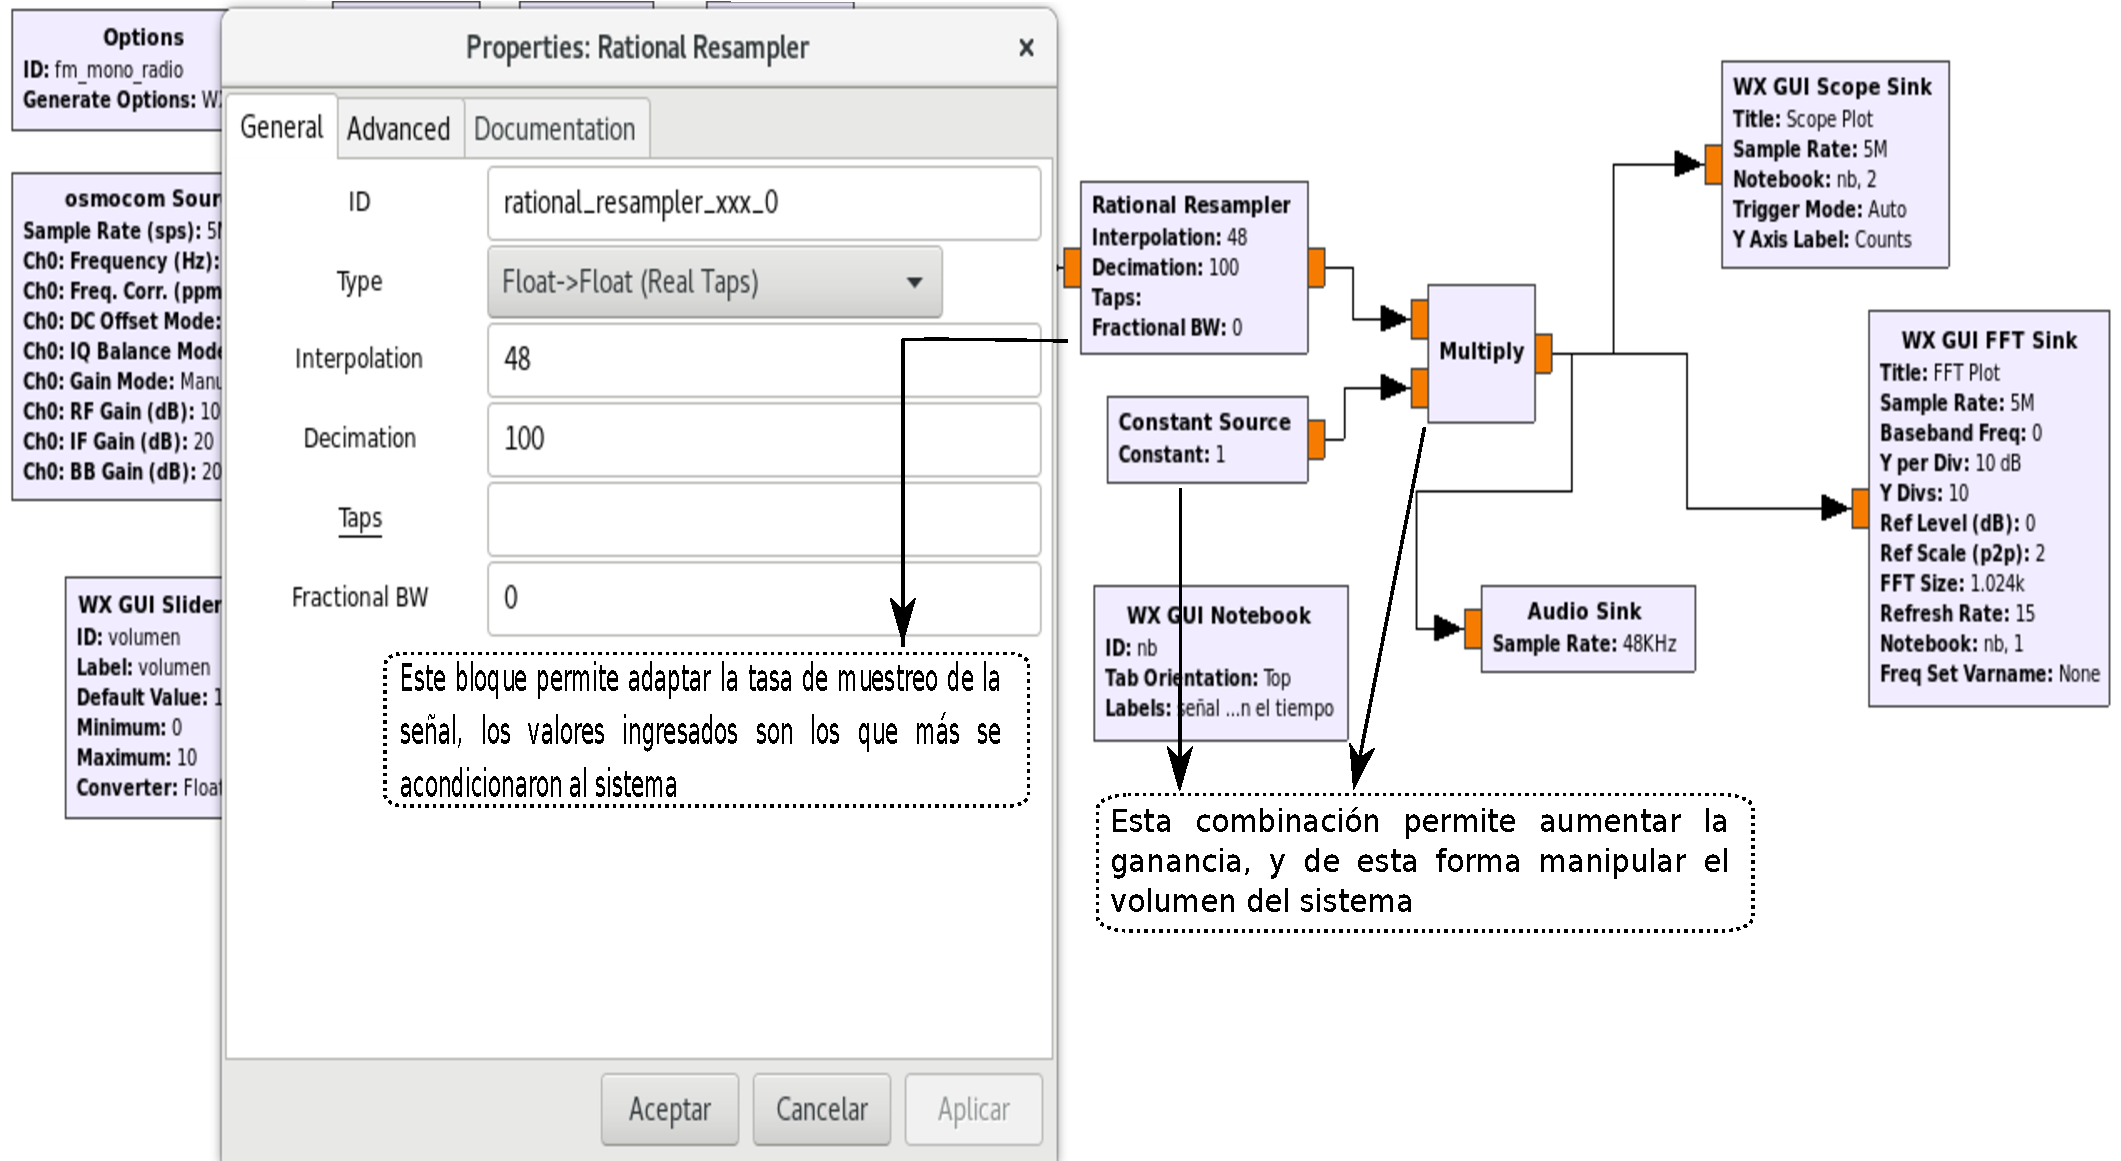
\includegraphics[width=\textwidth]{parte3/lab8/pdf/lab8_6.pdf}
\end{figure}

\end{frame}
%---------------------------------

\begin{frame}{Espectro señal recibida}

\begin{figure}[H]
\centering
\vspace{-3mm}
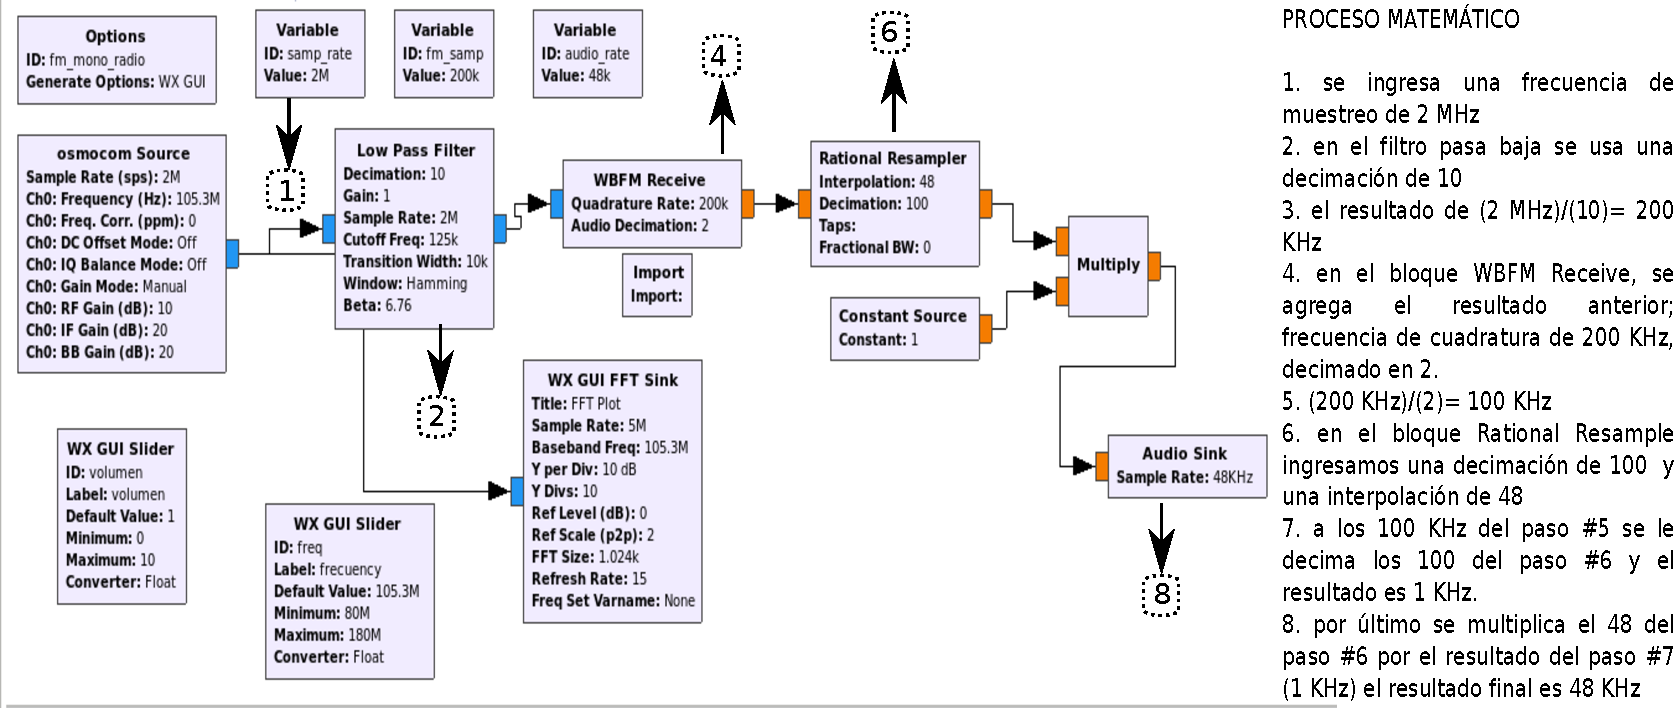
\includegraphics[width=\textwidth]{parte3/lab8/pdf/lab8_7.pdf}
\end{figure}

\end{frame}
%---------------------------------

\begin{frame}{Espectro señal demodulada}

\begin{figure}[H]
\centering
\vspace{-3mm}
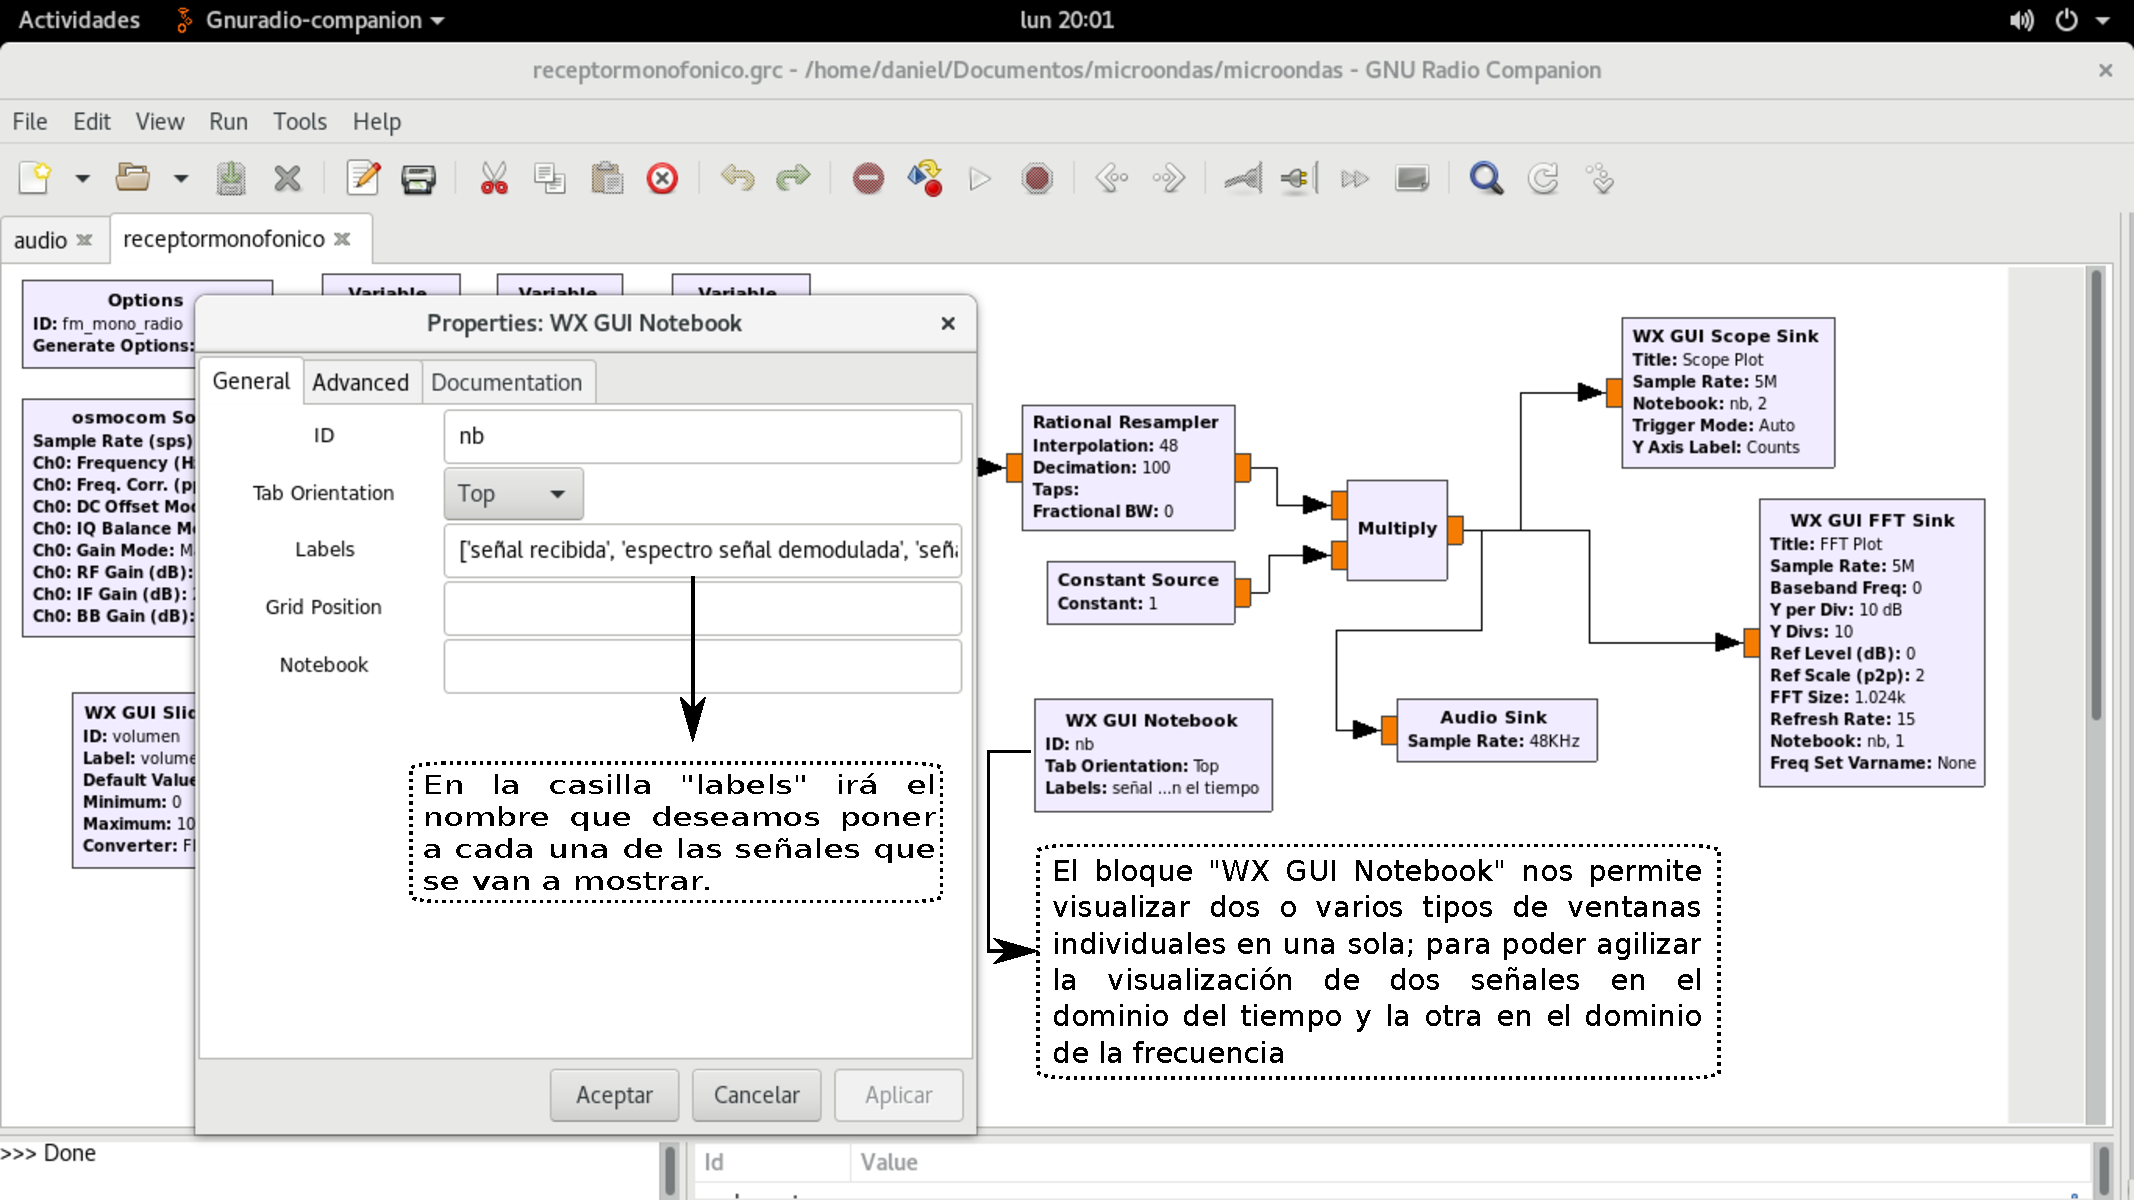
\includegraphics[width=\textwidth]{parte3/lab8/pdf/lab8_8.pdf}
\end{figure}

\end{frame}
%---------------------------------

\begin{frame}{Señal demodulada en tiempo}

\begin{figure}[H]
\centering
\vspace{-3mm}
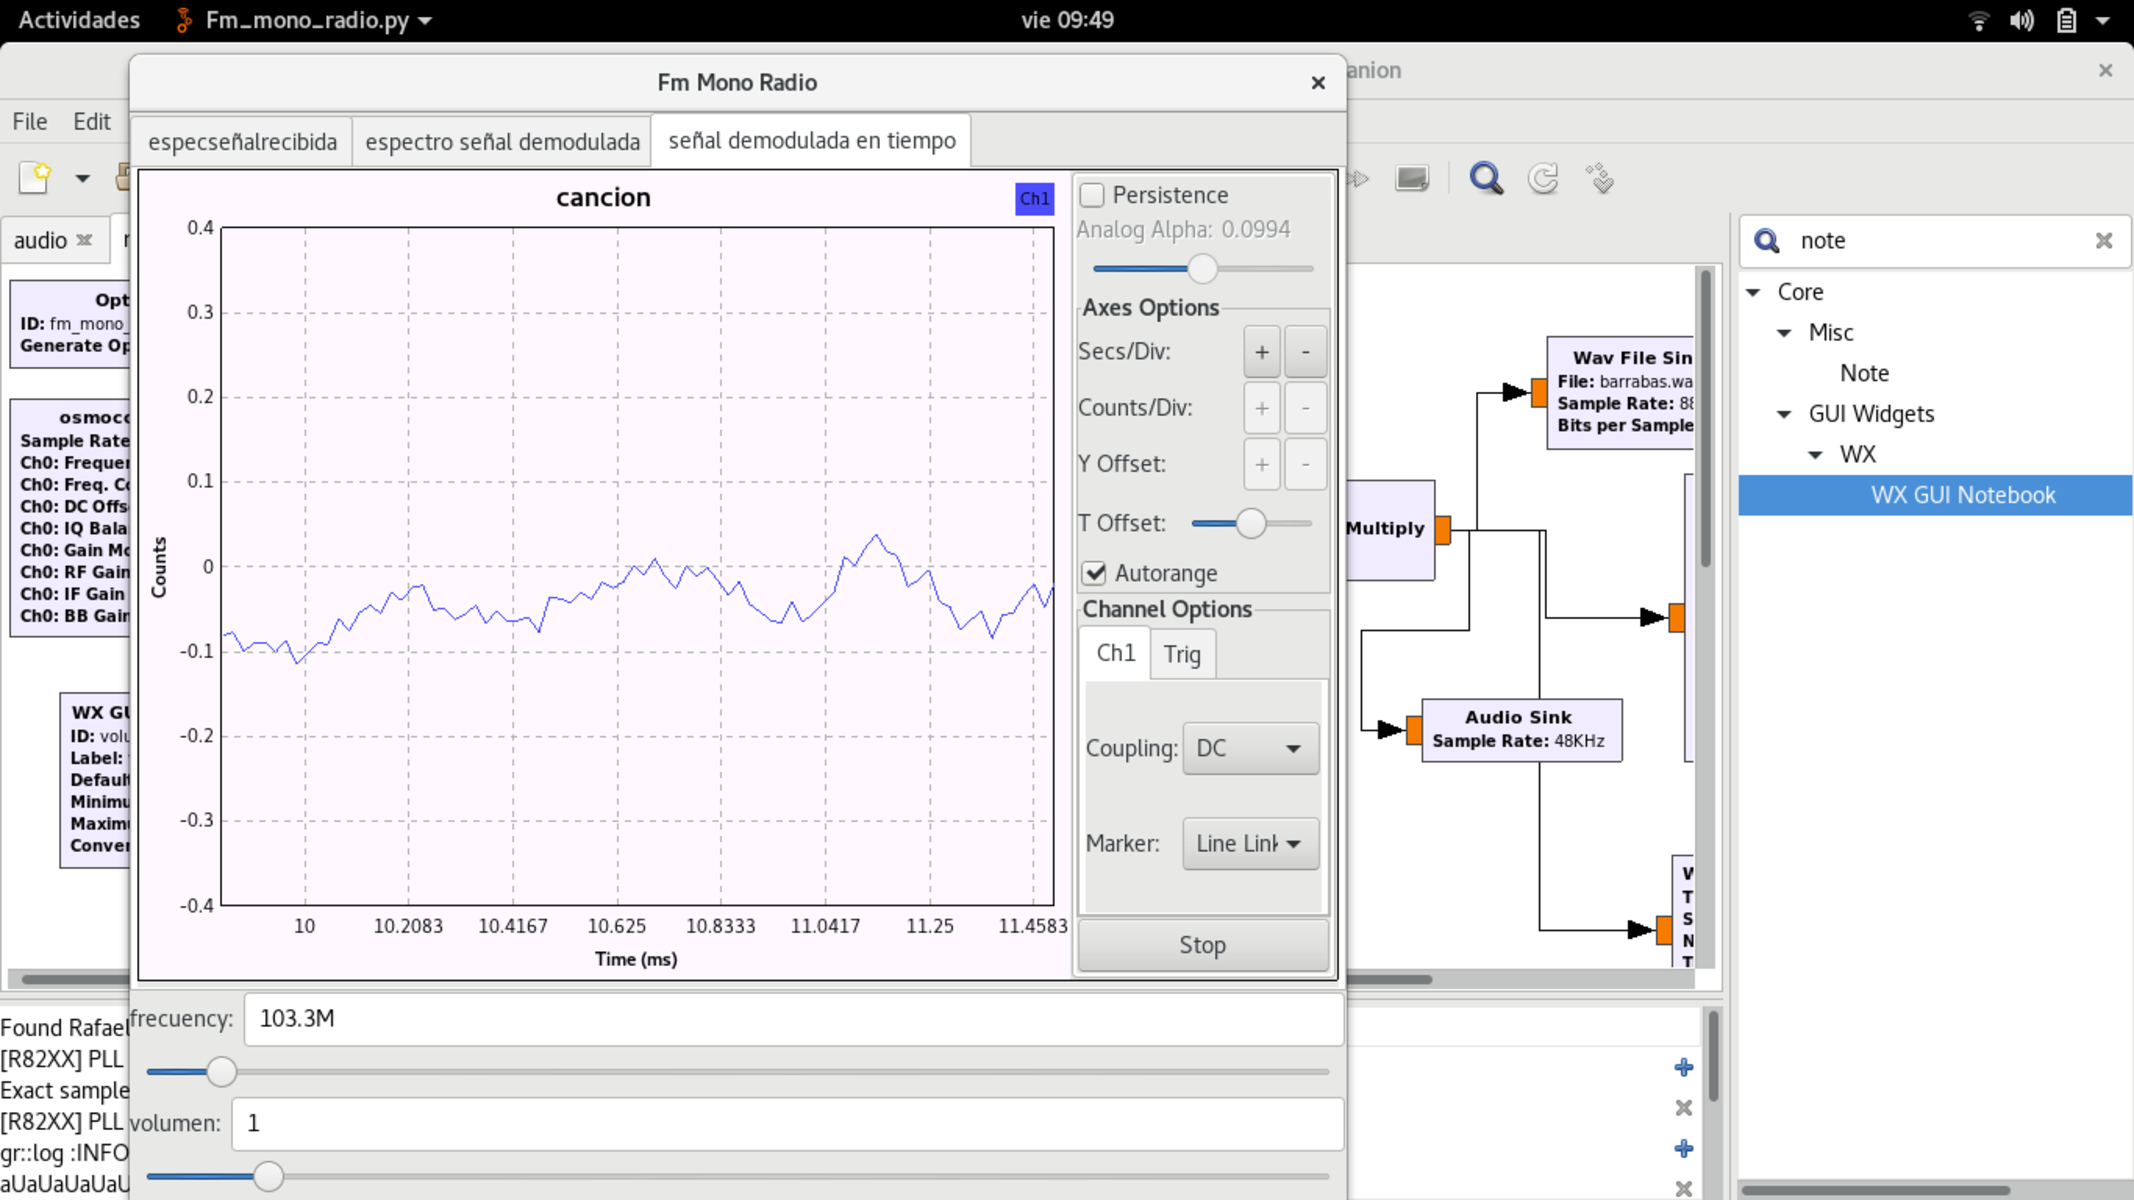
\includegraphics[width=\textwidth]{parte3/lab8/pdf/lab8_9.pdf}
\end{figure}

\end{frame}
%---------------------------------

